\begin{frame}{Beispiel für ein einfaches Gitterproblem}
    \textbf{Problemstellung:}
    \begin{itemize}
        \item Sei $\mathbf{g}_1, \dots, \mathbf{g}_k \in \mathbb{R}^n$ ein Set von Vektoren welche das Gitter $\mathcal{L}$ generieren
        \item Berechne eine Basis von $\mathbf{b}_1, \dots, \mathbf{b}_m \in \mathbb{R}^n$ von $\mathcal{L}$
        \item Bestimme, ob ein beliebiger Vektor ein Element vom Gitter $\mathcal{L}$ ist
    \end{itemize}
    \textbf{Lösungsansatz:}
    \begin{itemize}
        \item Basismatrize $\mathbf{B}$ mit dem Gauss-Algorithmus aus den $\mathbf{g}_i$ berechnen
        \item Das lineare Gleichungssystem lösen
        \item Der Vektor $\mathbf{c}$ ist genau dann ein Element von $\mathcal{L}$, wenn $\mathbf{x} \in \mathbb{Z}^m$ ist (alle Einträge ganzzahlig)
    \end{itemize}
    \note{
        Wieso ist das so? Das Gitter $\mathcal{L}$ besteht per Definition genau aus allen ganzzahligen Linearkombinationen der Basisvektoren,
        also $\mathcal{L} = \{\mathbf{B}\mathbf{x} : \mathbf{x} \in \mathbb{Z}^m\}$.
        Ein Vektor $\mathbf{c}$ liegt also genau dann im Gitter, wenn es ganzzahlige Koeffizienten $x_i$ gibt mit $\mathbf{c} = \mathbf{B}\mathbf{x}$.\newline
        \newline
        Nur wenn Fragen auftauchen:\newline
        Da die Basisvektoren linear unabhängig sind, hat das Gleichungssystem $\mathbf{B}\mathbf{x} = \mathbf{c}$ höchstens eine Lösung (über $\mathbb{R}$).
        Es gibt also keine andere Darstellung von $\mathbf{c}$, die ganzzahlig sein könnte, falls die berechnete Lösung nicht ganzzahlig ist.
        Ist $\mathbf{x}$ ganzzahlig, gilt $\mathbf{c} \in \mathcal{L}$, sonst $\mathbf{c} \notin \mathcal{L}$.\newline
    }
\end{frame}

\begin{frame}{Einfaches Gitterproblem: Beispiel mit Lösung}
    \textbf{Gegeben:}
    \[
        \mathbf{g}_1 = \begin{pmatrix} 2 \\ 0 \end{pmatrix},\;
        \mathbf{g}_2 = \begin{pmatrix} 1 \\ 2 \end{pmatrix},\;
        \mathbf{g}_3 = \begin{pmatrix} 3 \\ 2 \end{pmatrix}
        \qquad
        \qquad
        \mathbf{c}_1 = \begin{pmatrix} 5 \\ 2 \end{pmatrix},\;
        \mathbf{c}_2 = \begin{pmatrix} 4 \\ 2 \end{pmatrix}
    \]
    \textbf{Lösung:}
    \begin{itemize}
        \item Basis: $\mathbf{g}_3 = \mathbf{g}_1 + \mathbf{g}_2$ ist linear abhängig, also weglassen:
        $\mathbf{B} = \begin{pmatrix} 2 & 1 \\ 0 & 2 \end{pmatrix}$
        \item $\mathbf{c}_1$: $x_2 = 1$, $x_1 = 2$ \qquad also $\mathbf{x} = \begin{pmatrix} 2 \\ 1 \end{pmatrix} \in \mathbb{Z}^2$ \; $\Rightarrow$ $\mathbf{c}_1 \in \mathcal{L}$
        \item $\mathbf{c}_2$: $x_2 = 1$, $x_1 = \tfrac{3}{2}$ \qquad also $\mathbf{x} \notin \mathbb{Z}^2$ \; $\Rightarrow$ $\mathbf{c}_2 \notin \mathcal{L}$
    \end{itemize}
    \note{
        Laufzeit: Das Verfahren ist polynomiell, bei $k \approx n$ Erzeugern etwa $O(n^3)$ (Basisberechnung dominiert, Gleichungssystem lösen ist $O(n \cdot m^2)$).\newline
    }
\end{frame}

\begin{frame}{Shortest Vector Problem (SVP)~\textendash~... des kürzesten Vektors}
    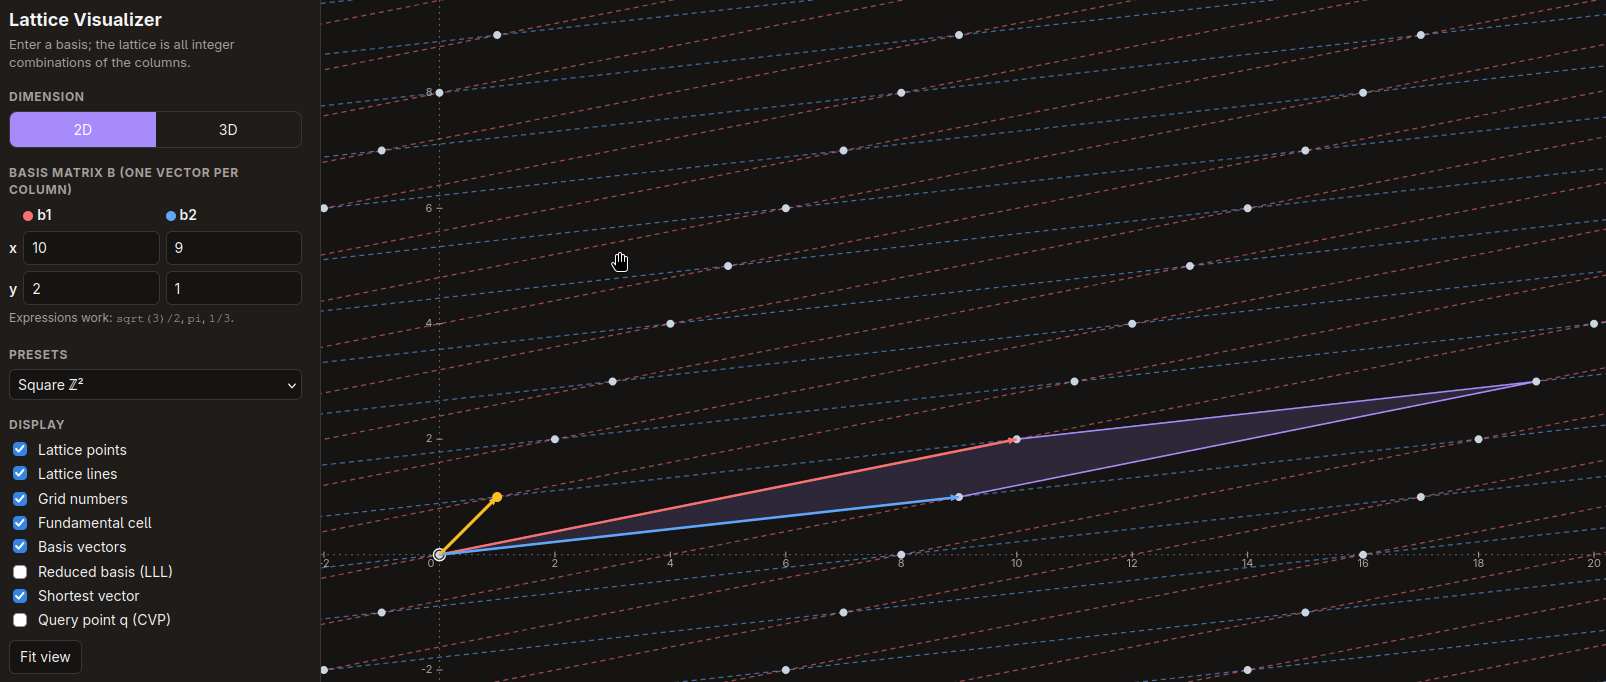
\includegraphics[width=\textwidth]{../assets/lattice_tool_shortest_vector_problem.png}
    \note{
        Vereinfacht gesagt beschreibt das Problem des kürzesten Vektors (kurz SVP) die Suche nach dem Vektor mit der kürzesten Distanz zum Nullpunkt/Uhrsprung.
    }
\end{frame}

\begin{frame}{Shortest Vector Problem (SVP): Definition}
    \begin{itemize}
        \item Sei $\mathcal{L}$ ein Gitter mit einer Basis $\mathbf{B} \in \mathbb{R}^{n \times m}$ und einer Norm $\|\cdot\|$.
        \item Sei $\lambda(\mathcal{L})$ die Länge des kürzesten Vektors ungleich null in $\mathcal{L}$.
        \item Die Aufgabe, ein $\mathbf{l} \in \mathcal{L}$ zu finden mit $\|\mathbf{l}\| = \lambda(\mathcal{L})$, also irgendeinen kürzesten Vektor von $\mathcal{L}$ zu finden, heisst \textit{Shortest Vector Problem (SVP)}.
    \end{itemize}
    \vspace{2em}
    {\setbeamerfont{itemize/enumerate body}{size=\footnotesize}
    \begin{itemize}
        \item NP-Schwer: z.B. Enumeration $2^{O(n \log n)}$
        \item LLL findet in polynomieller Zeit ein Resultat, dass max. $2^{O(n)}$ zu lang ist
    \end{itemize}
    }
    \note{
        SVP ist NP-schwer und exakte Algorithmen brauchen exponentielle Zeit in der Dimension $n$: Also etwas in der Form $2^{O(n \log n)}$, z.B. für die Enumeration.\newline
        \newline
        In polynomieller Zeit ist nur eine Näherung möglich: LLL findet einen Vektor, der höchstens um einen Faktor $2^{O(n)}$ länger ist als der kürzeste.
    }
\end{frame}

\begin{frame}{Closest Vector Problem (CVP)~\textendash~... des nächstgelegenen Vektors}
    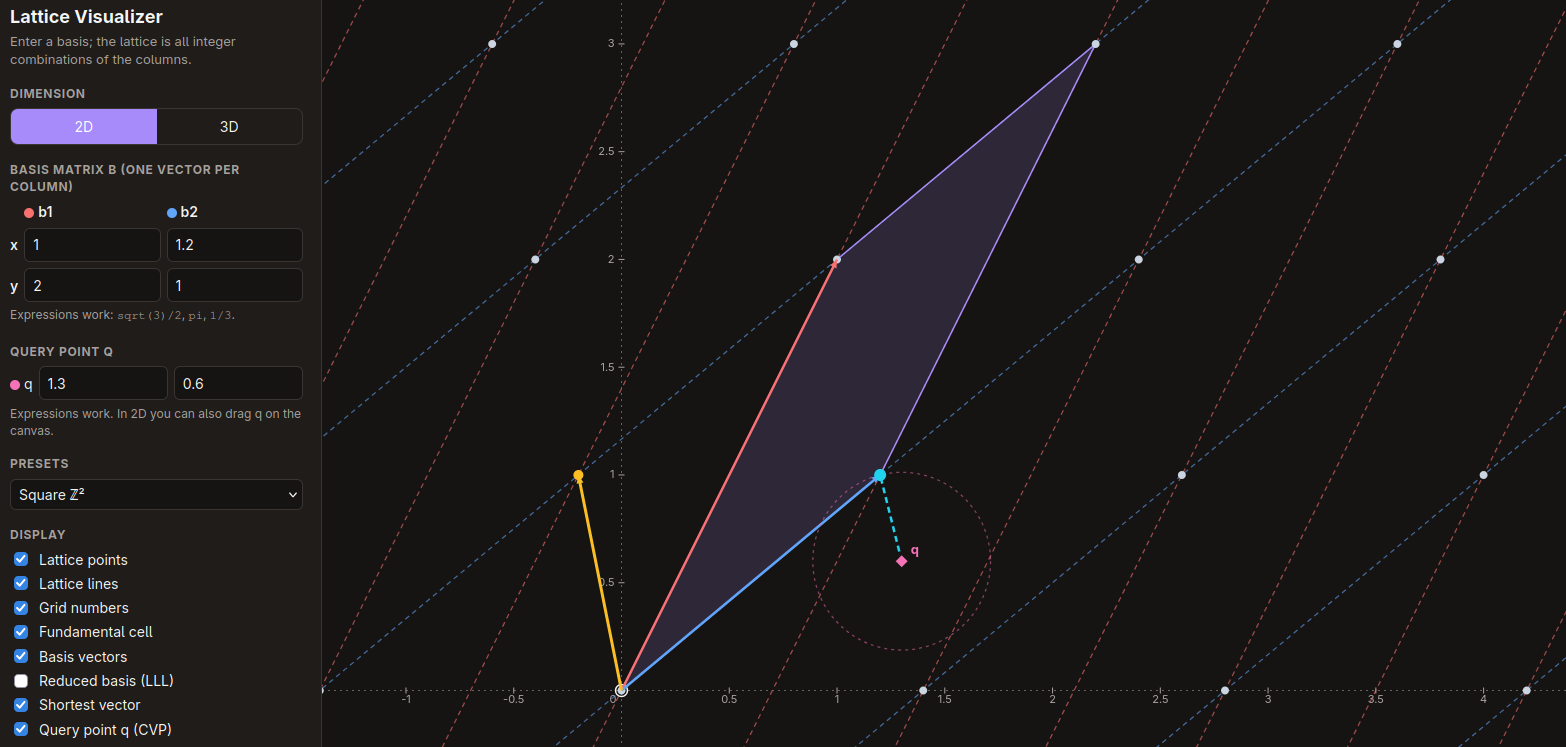
\includegraphics[width=\textwidth]{../assets/lattice_tool_closest_vector_problem.png}
    \note{
        Die Suche nach dem Vektor mit der kürzesten Distanz zu einem beliebig gewählten Punkt nennt man das Problem des nächstgelegenen Vektors (kurz CVP).
    }
\end{frame}

\begin{frame}{Closest Vector Problem (CVP): Definition}
    \begin{itemize}
        \item Sei $\mathcal{L}$ ein Gitter mit einer Basis $\mathbf{B} \in \mathbb{R}^{n \times m}$ und einer Norm $\|\cdot\|$ (Vektorlänge, üblicherweise die Euklidische Norm $\|\mathbf{v}\| = \sqrt{v_1^2 + \dots + v_n^2}$).
        \item Gegeben sei ein $\mathbf{q} \in \mathbb{R}^n$.
        \item Die Aufgabe, ein $\mathbf{l} \in \mathcal{L}$ zu finden, für das $\|\mathbf{l} - \mathbf{q}\|$ minimal ist, also den Gittervektor $\mathbf{l}$ zu finden, der einem beliebig vorgegebenen Vektor am nächsten liegt, heisst \textit{Closest Vector Problem (CVP)}.
    \end{itemize}
    \vspace{2em}
    {\setbeamerfont{itemize/enumerate body}{size=\footnotesize}
    \begin{itemize}
        \item NP-Schwer: mindestens so schwer wie SVP
        \item Babai-Algorithmus findet in polynomieller Zeit ein Resultat, dass max. $2^{O(n)}$ zu lang ist
    \end{itemize}
    }
    \note{
        Zur Geschätzte Laufzeit: CVP ist NP-schwer und gilt als mindestens so schwer wie SVP.\newline
        \newline
        In polynomieller Zeit geht nur eine Näherung, z.B. der Babai-Algorithmus auf einer LLL-reduzierten Basis mit einem Faktor $2^{O(n)}$.
    }
\end{frame}